\section{Teilversuch 1: Sichtbarmachen der Magnetfeldlinien mit Hilfe von Eisenspänen}
	\vfill
	\begin{multicols}{2}
		\begin{figure}[H]
			\centering
			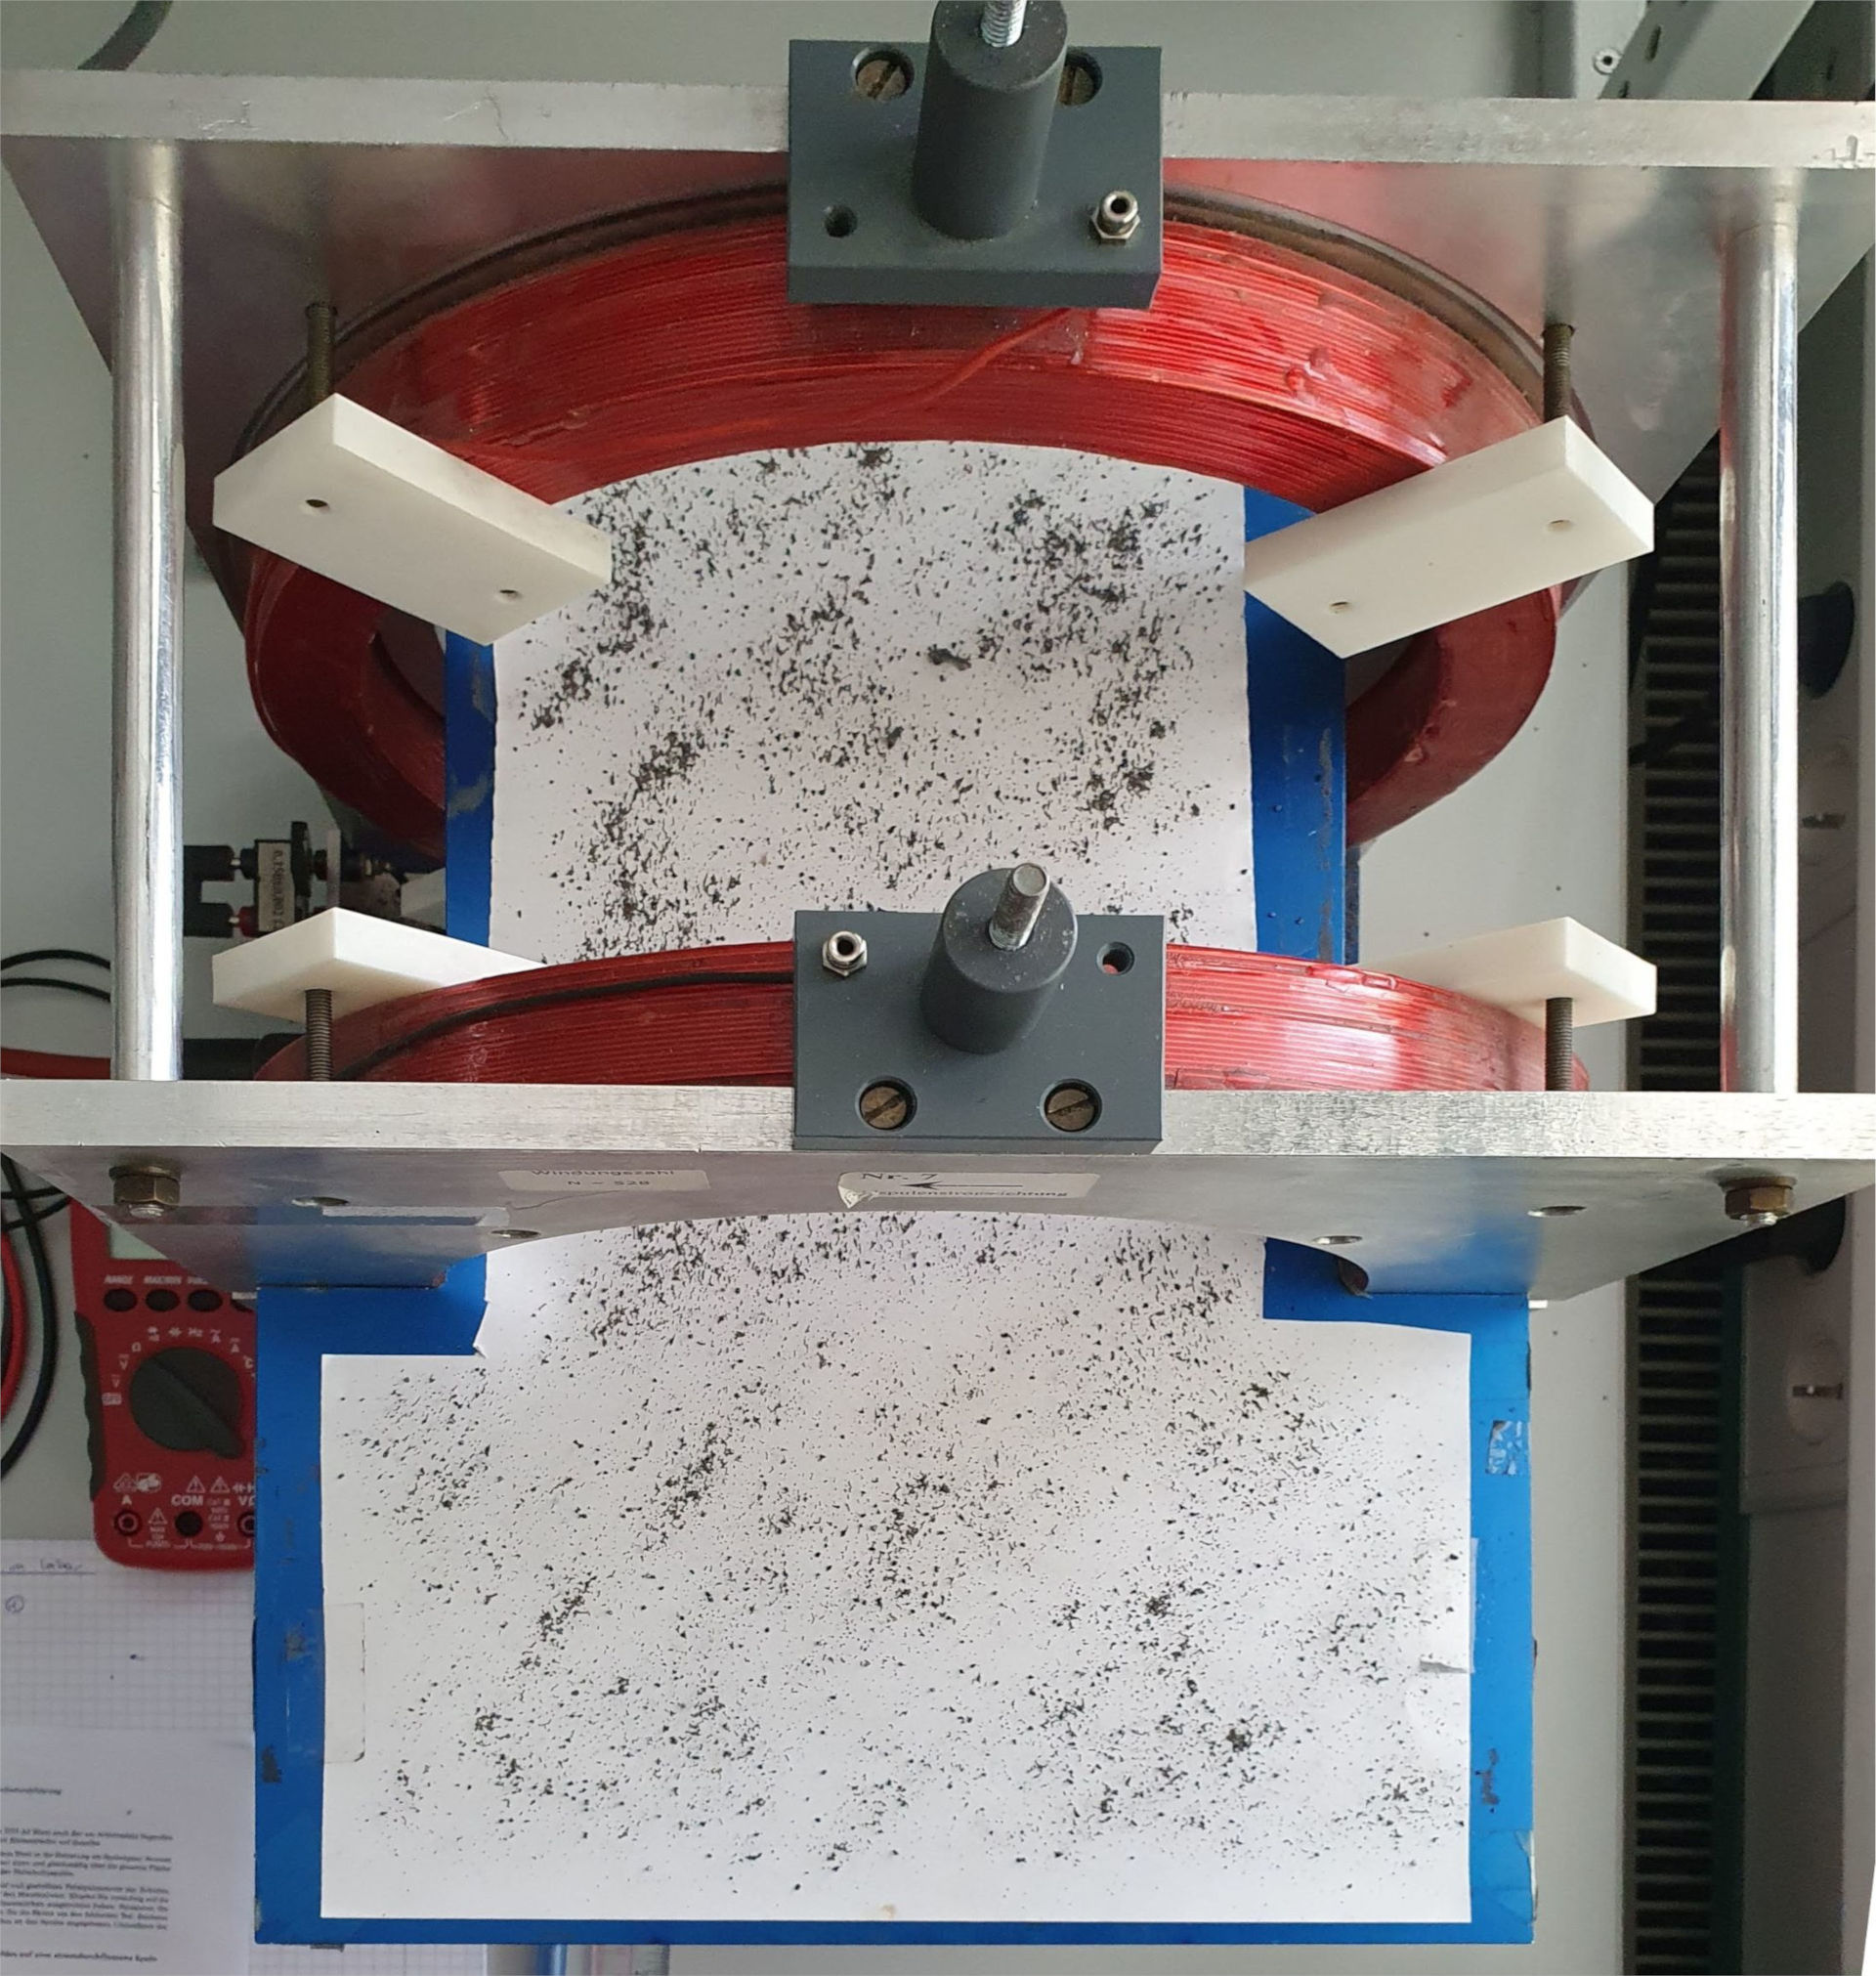
\includegraphics[width=0.4\textwidth]{./images/tv1-before-small.jpg}
			\caption{Ohne Magnetfeld}
		\end{figure}
		\begin{figure}[H]
			\centering
			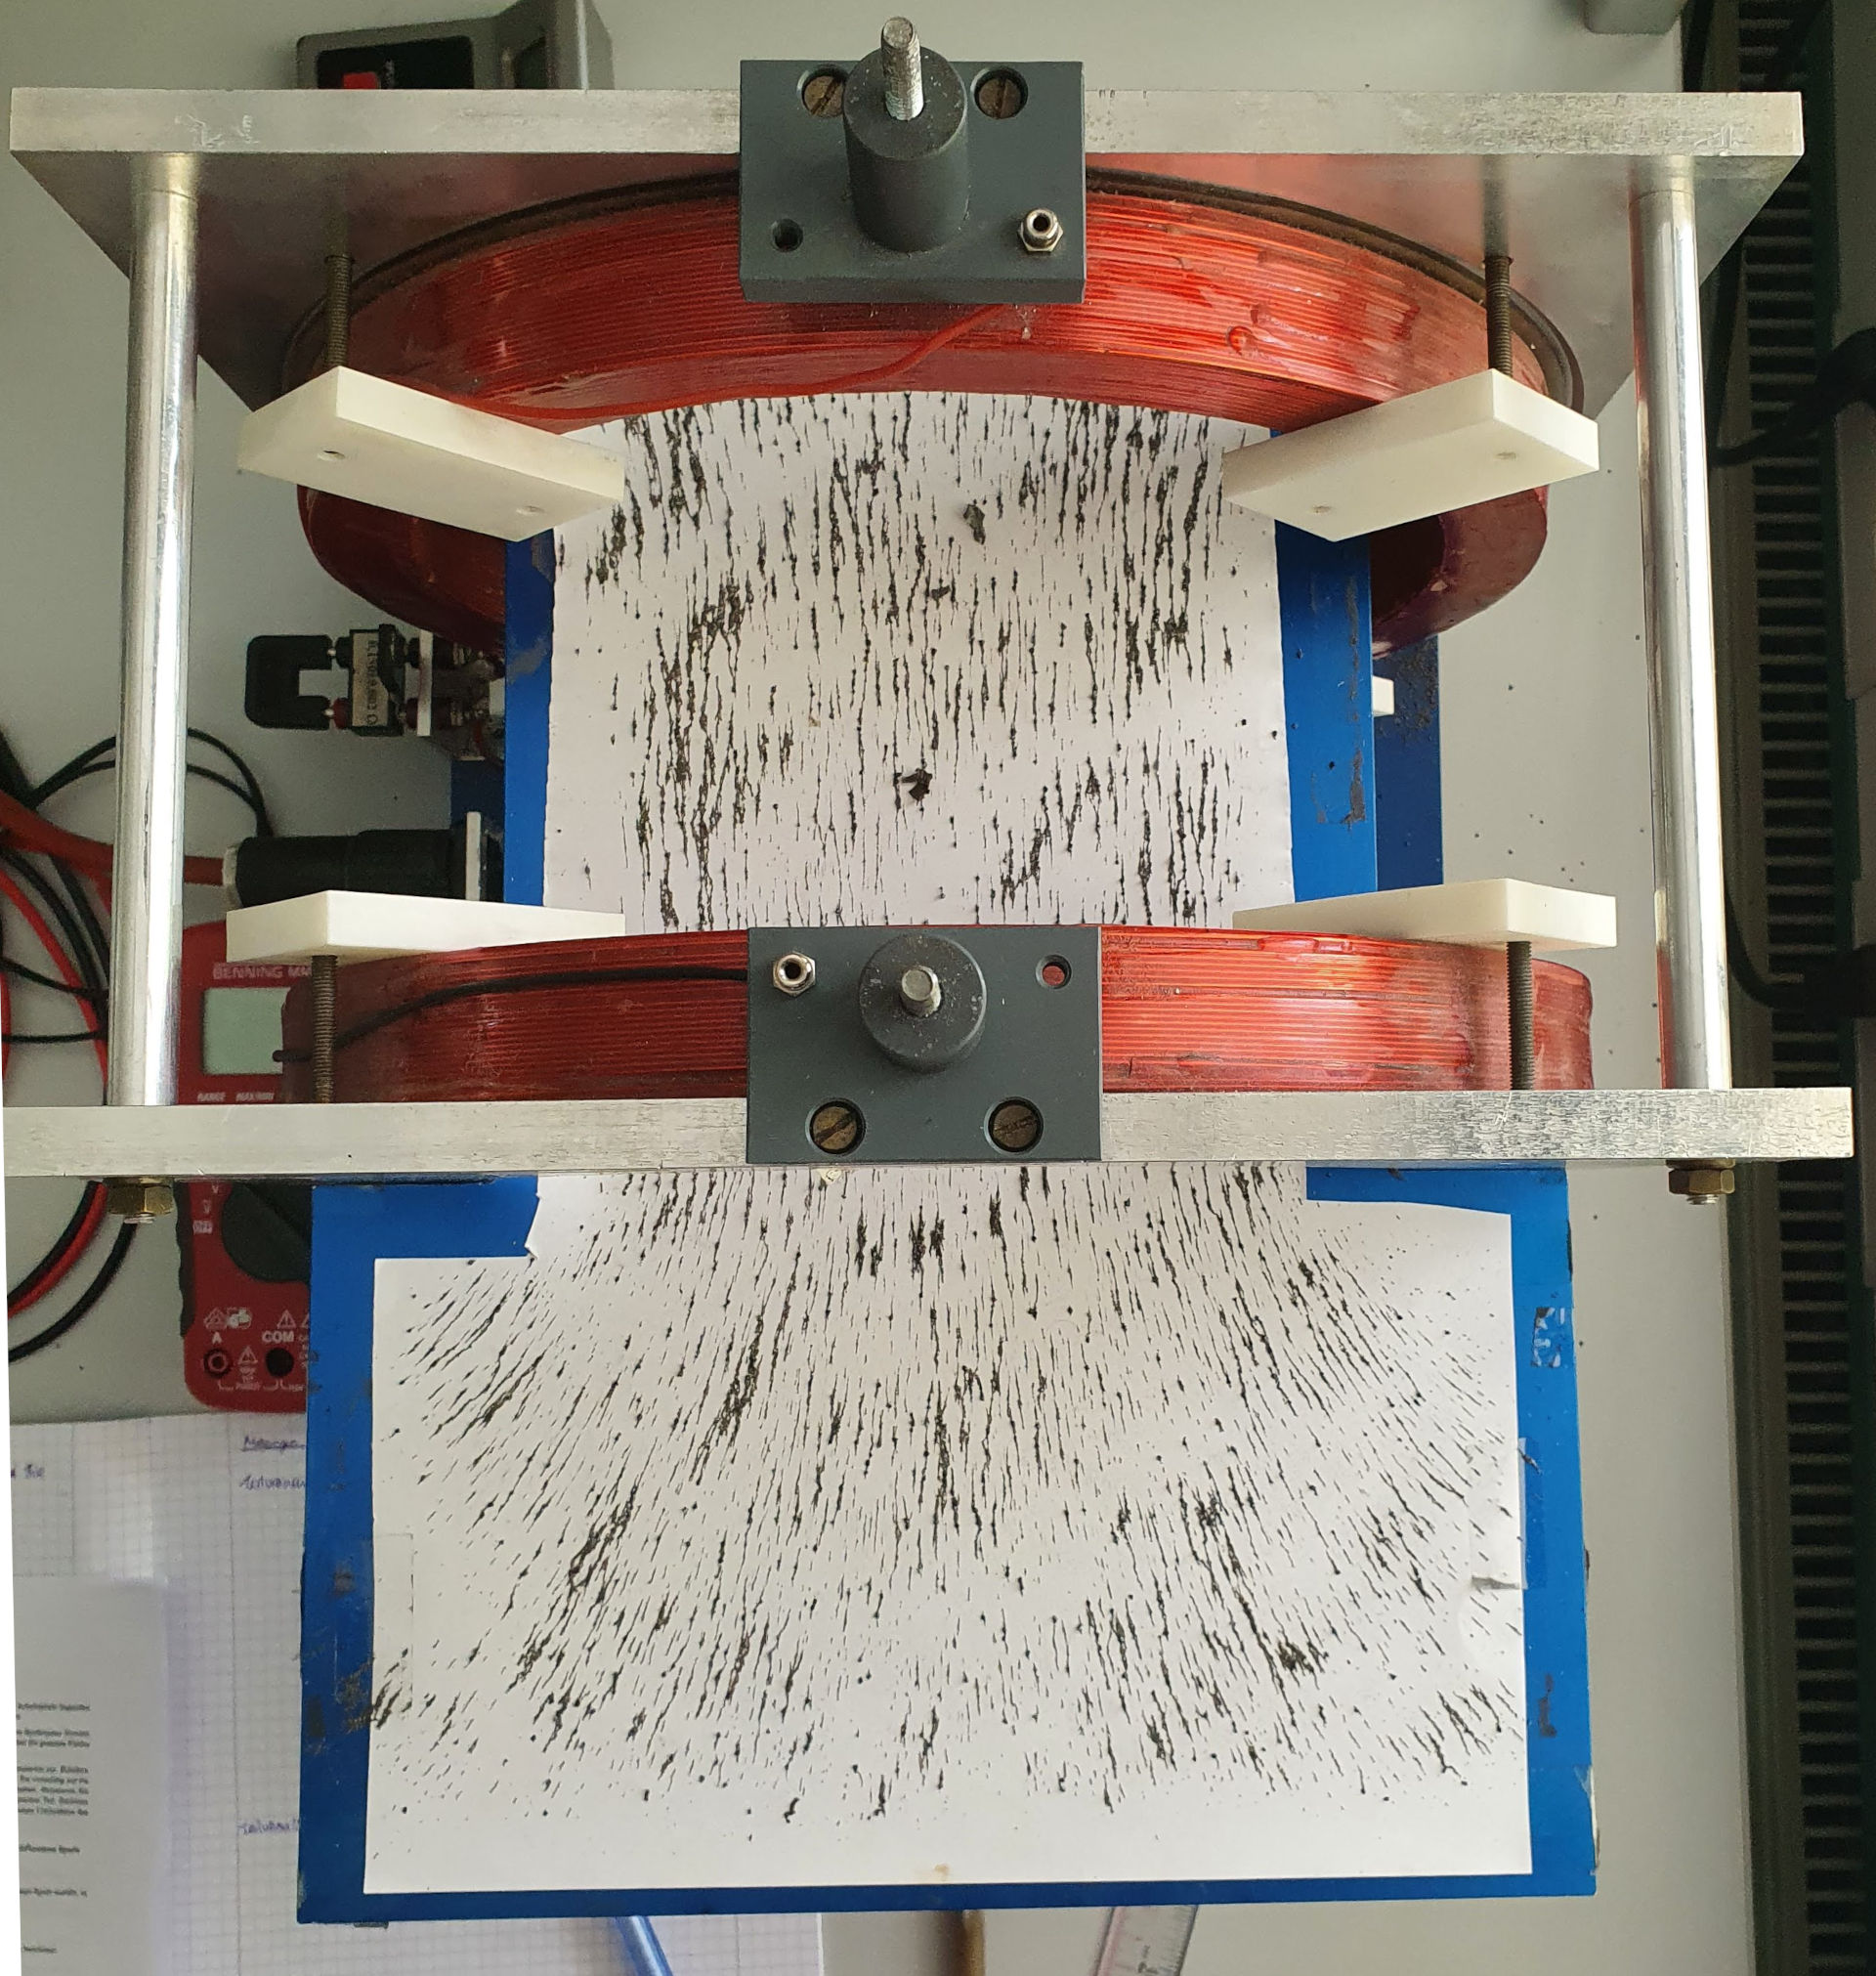
\includegraphics[width=0.4\textwidth]{./images/tv1-after-small.jpg}
			\caption{Mit Magnetfeld}
		\end{figure}
	\end{multicols}
	\vfill
